\section{Расчёт свойств потока}

В отличии от функций расчета PVT (физико-химических свойств флюидов) функции расчета свойства потока учитывают дополнительные параметры потока флюидов - $Q$ - дебит, объемный расход флюидов, $f_w$ - обводненность, $R_p$ - газовый фактор. В функциях свойств потока используется префикс \mintinline{vb.net}{feed_}.

Параметры потока, такие как расход ГЖС, доля газа в потоке, вязкость ГЖС важны для расчёта и анализа работы скважин и скважинного оборудования.


\subsection{feed\_q\_mix\_rc\_m3day – расход газожидкостной смеси}

Функция позволяет рассчитать объёмный расход газожидкостной смеси при заданных термобарических условиях. Объёмный расход ГЖС важен например для подбора УЭЦН в скважине, так как именно определяет в какой точке характеристики УЭЦН будет работать. При наличии свободного газа в потоке расход ГЖС может быть значительно больше расхода жидкости на поверхности фиксируемого расходомером.
$$Q_{mix,rc} = Q_{w,sc} B_w(P,T) + Q_{o,sc} B_o(P,T)  + Q_{o,sc}  (R_p - R_s(P,T)) B_g(P,T) $$

Расход ГЖС определяется как сумма расходов отдельных фаз, приведённых к соответствующим термобарическим условиям, с учётом того, что часть газа будет растворена в нефти.

\putlisting{listings/feed_q_mix_rc_m3day.lst}

\subsection{feed\_rho\_mix\_kgm3 – плотность газожидкостной смеси}

Функция позволяет рассчитать плотность газожидкостной смеси при заданных термобарических условиях. 
$$\rho_{mix,rc} = \left( \frac{\rho_{w,sc}}{B_w} f_w + \frac{\rho_{o,sc} +r_s \rho_{g,sc} }{B_o}(1-f_w) \right) (1-f_g) + \frac{ \rho_{g,sc} }{B_g} f_g $$

\putlisting{listings/feed_rho_mix_kgm3.lst}

\subsection{feed\_gas\_fraction\_d – доля газа в потоке}

Функция расчёта доли свободного газа в потоке (без учёта проскальзывания) в зависимости от термобарических условий для заданного флюида. 
$$f_g = \frac{Q_{gas\_rc} (1-k_{sep\_add})}{Q_{wat\_rc}+Q_{oil\_rc}+Q_{gas\_rc}(1-k_{sep\_add})} $$
где все объёмные расходы фаз приведены в соответствующих термобарических условиях, а $k_{sep,add}$ - дополнительный коэффициент сепарации, учитывающий удаление части свободного газа из потока.

Доля газа в потоке является одним из ключевых параметров ограничивающих производительность систем механизированной добычи - ЭЦН и других насосов.

\putlisting{listings/feed_gas_fraction_d.lst}

\subsection{feed\_p\_gas\_fraction\_atma – целевое давления для заданной доли газа в потоке}
Функция расчёта давления при котором достигается заданная доля свободного газа в потоке (без учёта проскальзывания). 
Значение давления при котором достигается определённая доля газа в потоке может быть найдено из решения уравнения, определяющего долю газа. 
$$f_g = \frac{Q_{gas\_rc} (1-k_{sep\_add})}{Q_{wat\_rc}+Q_{oil\_rc}+Q_{gas\_rc}(1-k_{sep\_add})} $$
Решение в \unf{} реализовано итеративное, методом деления отрезка пополам (дихотомия). При вызове функции пересчитывается состояние смеси с различными термобарическими условиями. Поэтому расчёт проводится относительно медленно. 

Задание $k_{sep\_add}$ позволит оценить целевое давление на приеме для ЭЦН при известной доли газа и известном ожидаемом значении сепарации газа. Отметим, что значение сепарации может быть оценено по корреляционным зависимостям. Но такие зависимости требуют знания давления сепарации, а следовательно их учет совместно с алгоритмом расчета давления при котором достигается определенная доля газа потребует итеративного решения, что выходит за рамки данной функции (например из за того, что это потребует задания дополнительных параметров конфигурации скважины).

\putlisting{listings/feed_p_gas_fraction_atma.lst}



\subsection{feed\_rp\_gas\_fraction\_m3m3 – целевой газовый фактор для заданной доли газа в потоке}
Функция расчёта газового фактора $R_p$ при котором достигается заданная доля свободного газа в потоке (без учёта проскальзывания) . 
Значение давления при котором достигается определённая доля газа в потоке может быть найдено из решения уравнения, определяющего долю газа. 
$$f_g = \frac{Q_{gas\_rc} (1-k_{sep\_add})}{Q_{wat\_rc}+Q_{oil\_rc}+Q_{gas\_rc}(1-k_{sep\_add})} $$

Решение в \unf{} реализовано с использованием итераций, методом деления отрезка пополам (дихотомия). При вызове функции  состояние смеси пересчитывается с различными термобарическими условиями. Поэтому расчёт проводится относительно медленно. 

Задание $k_{sep\_add}$ позволит оценить целевой газовый фактор при известной доли газа, давлении на приеме и ожидаемом значении сепарации газа. Отметим, что значение сепарации может быть оценено по корреляционным зависимостям. Но такие зависимости требуют знания как давления сепарации так и газового фактора, а следовательно их учет совместно с алгоритмом расчета газового фактора при котором достигается определенная доля газа потребует итеративного решения, что выходит за рамки данной функции (например из за того, что это потребует задания дополнительных параметров конфигурации скважины).

\putlisting{listings/feed_rp_gas_fraction_m3m3.lst}

\section{Сепарация газа в скважине}
В скважинах оборудованных системами механизированной добычи нефти важную роль играет процесс сепарации газа на приёме насоса. Под сепарацией газа понимается отделение части свободного газа из потока и перенаправление его по отдельному гидравлическому каналу на поверхность. В результате сепарации газа меняются свойства флюида, поступающего в насос и НКТ выше насоса. В частности меняются давление насыщения и газосодержание при давлении насыщения для флюида после сепарации. Более детальные модели флюида и сепарации могут показать, что при сепарации может поменяться и другие параметры - например состав газа после разгазирования. В модели нелетучей нефти реализованной в \unf{} эти эффекты не учитываются.


\begin{figure}[H]
	\centering
		

\tikzset{every picture/.style={line width=0.75pt}} %set default line width to 0.75pt        

\begin{tikzpicture}[x=0.75pt,y=0.75pt,yscale=-1,xscale=1]
%uncomment if require: \path (0,406); %set diagram left start at 0, and has height of 406

%Shape: Rectangle [id:dp04480742808021354] 
\draw  [fill={rgb, 255:red, 155; green, 155; blue, 155 }  ,fill opacity=1 ] (312,64.14) -- (351.5,64.14) -- (351.5,114.5) -- (312,114.5) -- cycle ;
%Shape: Rectangle [id:dp3210354209072095] 
\draw  [line width=2.25]  (259.42,64.14) -- (404.08,64.14) -- (404.08,352) -- (259.42,352) -- cycle ;
%Shape: Rectangle [id:dp11917689807401133] 
\draw  [fill={rgb, 255:red, 155; green, 155; blue, 155 }  ,fill opacity=1 ] (296.75,114.5) -- (366.75,114.5) -- (366.75,314.5) -- (296.75,314.5) -- cycle ;
%Shape: Rectangle [id:dp22447305445205257] 
\draw  [fill={rgb, 255:red, 255; green, 255; blue, 255 }  ,fill opacity=1 ] (305.89,238.94) -- (310.33,238.94) -- (310.33,269.56) -- (305.89,269.56) -- cycle ;
%Shape: Rectangle [id:dp05751039520762724] 
\draw  [fill={rgb, 255:red, 255; green, 255; blue, 255 }  ,fill opacity=1 ] (314.33,238.94) -- (318.78,238.94) -- (318.78,269.56) -- (314.33,269.56) -- cycle ;
%Shape: Rectangle [id:dp6083474962263296] 
\draw  [fill={rgb, 255:red, 255; green, 255; blue, 255 }  ,fill opacity=1 ] (322.11,238.94) -- (326.56,238.94) -- (326.56,269.56) -- (322.11,269.56) -- cycle ;
%Shape: Rectangle [id:dp9699991258462393] 
\draw  [fill={rgb, 255:red, 255; green, 255; blue, 255 }  ,fill opacity=1 ] (329.53,238.94) -- (333.97,238.94) -- (333.97,269.56) -- (329.53,269.56) -- cycle ;
%Shape: Rectangle [id:dp5276274421172025] 
\draw  [fill={rgb, 255:red, 255; green, 255; blue, 255 }  ,fill opacity=1 ] (337,238.94) -- (341.44,238.94) -- (341.44,269.56) -- (337,269.56) -- cycle ;
%Shape: Rectangle [id:dp8686039431642814] 
\draw  [fill={rgb, 255:red, 255; green, 255; blue, 255 }  ,fill opacity=1 ] (344.78,238.94) -- (349.22,238.94) -- (349.22,269.56) -- (344.78,269.56) -- cycle ;
%Shape: Rectangle [id:dp024923249699371652] 
\draw  [fill={rgb, 255:red, 255; green, 255; blue, 255 }  ,fill opacity=1 ] (352.56,238.94) -- (357,238.94) -- (357,269.56) -- (352.56,269.56) -- cycle ;
%Shape: Rectangle [id:dp24614630976896423] 
\draw  [fill={rgb, 255:red, 255; green, 255; blue, 255 }  ,fill opacity=1 ] (360.11,238.94) -- (364.56,238.94) -- (364.56,269.56) -- (360.11,269.56) -- cycle ;
%Shape: Rectangle [id:dp4580617305504924] 
\draw  [fill={rgb, 255:red, 255; green, 255; blue, 255 }  ,fill opacity=1 ] (298.78,238.94) -- (303.22,238.94) -- (303.22,269.56) -- (298.78,269.56) -- cycle ;
%Curve Lines [id:da46150758694693694] 
\draw [color={rgb, 255:red, 74; green, 144; blue, 226 }  ,draw opacity=1 ]   (282.2,352) .. controls (281.45,261.49) and (287.15,263.11) .. (299.52,257.34) ;
\draw [shift={(302.2,256)}, rotate = 511.33] [fill={rgb, 255:red, 74; green, 144; blue, 226 }  ,fill opacity=1 ][line width=0.08]  [draw opacity=0] (10.72,-5.15) -- (0,0) -- (10.72,5.15) -- (7.12,0) -- cycle    ;
%Shape: Circle [id:dp04721201185159396] 
\draw  [fill={rgb, 255:red, 255; green, 255; blue, 255 }  ,fill opacity=1 ] (304.99,174.01) .. controls (306.3,170.48) and (308.78,169.68) .. (310.52,172.22) .. controls (312.26,174.75) and (312.61,179.67) .. (311.3,183.19) .. controls (309.99,186.72) and (307.51,187.52) .. (305.77,184.98) .. controls (304.03,182.45) and (303.68,177.53) .. (304.99,174.01) -- cycle ;
%Shape: Circle [id:dp5883852152967295] 
\draw  [fill={rgb, 255:red, 255; green, 255; blue, 255 }  ,fill opacity=1 ] (350.59,174.01) .. controls (351.9,170.48) and (354.38,169.68) .. (356.12,172.22) .. controls (357.86,174.75) and (358.21,179.67) .. (356.9,183.19) .. controls (355.59,186.72) and (353.11,187.52) .. (351.37,184.98) .. controls (349.63,182.45) and (349.28,177.53) .. (350.59,174.01) -- cycle ;
%Curve Lines [id:da5619628529147929] 
\draw [color={rgb, 255:red, 74; green, 144; blue, 226 }  ,draw opacity=1 ]   (308.54,178.6) .. controls (288.8,173.65) and (285.1,176) .. (286.11,97.21) ;
\draw [shift={(286.14,94.8)}, rotate = 450.78] [fill={rgb, 255:red, 74; green, 144; blue, 226 }  ,fill opacity=1 ][line width=0.08]  [draw opacity=0] (10.72,-5.15) -- (0,0) -- (10.72,5.15) -- (7.12,0) -- cycle    ;
%Curve Lines [id:da7420889905281607] 
\draw [color={rgb, 255:red, 74; green, 144; blue, 226 }  ,draw opacity=1 ]   (269.4,352) .. controls (268.97,261.5) and (271.07,125.81) .. (271.01,97.45) ;
\draw [shift={(271,94.8)}, rotate = 449.4] [fill={rgb, 255:red, 74; green, 144; blue, 226 }  ,fill opacity=1 ][line width=0.08]  [draw opacity=0] (10.72,-5.15) -- (0,0) -- (10.72,5.15) -- (7.12,0) -- cycle    ;
%Curve Lines [id:da1955664158849284] 
\draw [color={rgb, 255:red, 74; green, 144; blue, 226 }  ,draw opacity=1 ]   (331.75,231.56) .. controls (331.45,207.23) and (331.44,241.87) .. (331.75,97) ;
\draw [shift={(331.75,94.8)}, rotate = 450.12] [fill={rgb, 255:red, 74; green, 144; blue, 226 }  ,fill opacity=1 ][line width=0.08]  [draw opacity=0] (10.72,-5.15) -- (0,0) -- (10.72,5.15) -- (7.12,0) -- cycle    ;
%Curve Lines [id:da5073323315189147] 
\draw [color={rgb, 255:red, 74; green, 144; blue, 226 }  ,draw opacity=1 ]   (331.75,230.44) .. controls (330.74,183.59) and (324.76,182.05) .. (316.18,179.48) ;
\draw [shift={(313.4,178.58)}, rotate = 379.94] [fill={rgb, 255:red, 74; green, 144; blue, 226 }  ,fill opacity=1 ][line width=0.08]  [draw opacity=0] (10.72,-5.15) -- (0,0) -- (10.72,5.15) -- (7.12,0) -- cycle    ;
%Curve Lines [id:da18312163514470803] 
\draw [color={rgb, 255:red, 74; green, 144; blue, 226 }  ,draw opacity=1 ]   (331.75,231.17) .. controls (330.77,185.6) and (339.02,182.33) .. (345.86,179.93) ;
\draw [shift={(348.56,178.89)}, rotate = 514.89] [fill={rgb, 255:red, 74; green, 144; blue, 226 }  ,fill opacity=1 ][line width=0.08]  [draw opacity=0] (10.72,-5.15) -- (0,0) -- (10.72,5.15) -- (7.12,0) -- cycle    ;
%Curve Lines [id:da5609474333970248] 
\draw [color={rgb, 255:red, 74; green, 144; blue, 226 }  ,draw opacity=1 ]   (353.74,178.6) .. controls (374.5,175.74) and (380.34,176.04) .. (381.54,97.21) ;
\draw [shift={(381.57,94.8)}, rotate = 450.78] [fill={rgb, 255:red, 74; green, 144; blue, 226 }  ,fill opacity=1 ][line width=0.08]  [draw opacity=0] (10.72,-5.15) -- (0,0) -- (10.72,5.15) -- (7.12,0) -- cycle    ;
%Curve Lines [id:da942989625089206] 
\draw [color={rgb, 255:red, 74; green, 144; blue, 226 }  ,draw opacity=1 ]   (394.29,352) .. controls (393.86,261.5) and (394.33,125.81) .. (394.16,97.45) ;
\draw [shift={(394.14,94.8)}, rotate = 449.4] [fill={rgb, 255:red, 74; green, 144; blue, 226 }  ,fill opacity=1 ][line width=0.08]  [draw opacity=0] (10.72,-5.15) -- (0,0) -- (10.72,5.15) -- (7.12,0) -- cycle    ;
%Curve Lines [id:da2534809401724647] 
\draw [color={rgb, 255:red, 74; green, 144; blue, 226 }  ,draw opacity=1 ]   (381.98,352) .. controls (381.21,259.56) and (377.98,263.5) .. (358.91,258.24) ;
\draw [shift={(356.11,257.42)}, rotate = 377.19] [fill={rgb, 255:red, 74; green, 144; blue, 226 }  ,fill opacity=1 ][line width=0.08]  [draw opacity=0] (10.72,-5.15) -- (0,0) -- (10.72,5.15) -- (7.12,0) -- cycle    ;
%Shape: Rectangle [id:dp25186132731738486] 
\draw  [color={rgb, 255:red, 255; green, 255; blue, 255 }  ,draw opacity=1 ][fill={rgb, 255:red, 255; green, 255; blue, 255 }  ,fill opacity=1 ] (249.86,58.29) -- (411.29,58.29) -- (411.29,70.29) -- (249.86,70.29) -- cycle ;
%Shape: Rectangle [id:dp3766484711992675] 
\draw  [color={rgb, 255:red, 255; green, 255; blue, 255 }  ,draw opacity=1 ][fill={rgb, 255:red, 255; green, 255; blue, 255 }  ,fill opacity=1 ] (251.43,346.29) -- (414.71,346.29) -- (414.71,358.57) -- (251.43,358.57) -- cycle ;





\end{tikzpicture}
		\caption{Схема линий тока газа на приеме ЭЦН}
		\label{ris:separation_scheme}
\end{figure}

В скважине с ЭЦН работают два механизма сепарации свободного газа из потока, схематично показанные на рисунке \ref{ris:separation_scheme} - естественная или натуральная сепарация газа, когда часть свободного газа за счет сил всплытия проходит мимо приема насоса и искусственная сепарация с применением газосепаратора, когда часть свободного газа выталкивается из насоса, обычно за счет центробежных сил. 

Оценка этих механизмов, а также расчёт общей сепарации могут быть проведены приведёнными ниже функциями.

\subsection{well\_ksep\_natural\_d – естественная сепарация газа}
Функция рассчитывает естественную сепарацию газа на приёме насоса в скважине с использованием корреляции Маркеса \cite{Marquez_2003} . Результат - безразмерная величина в диапазоне от 0 до 1. 

\putlisting{listings/well_ksep_natural_d.lst}

%\subsection{ESP\_ksep\_gasseparator\_d – сепарация газа роторным газосепаратором}
%Функция рассчитывает сепарацию газа с использованием роторного газосепаратора, являющегося обычно частью компоновки УЭЦН. Данный расчет основан на результатах испытания характеристик роторных газосепараторов, выполненных в РГУ нефти и газа имени И.М.Губкина \cite{SPE_117415_2008}. 

%Следует отметить, что несмотря на хорошее соответствие промысловых исследований и расчетов с использованием корреляции для естественной и искусственной сепарации \cite{SPE_117415_2008} к результатам стендовых исследований стоит относится с осторожностью. Основой осторожности могут быть следующие соображения: характеристики различных газосепараторов достаточно сильно отличаются друг от друга - есть удачные конструкции и не очень, при этом результаты стендовых испытаний доступны только для ограниченного набора конструкций, стендовые условия достаточно сильно отличаются от скважинных - ниже давление, другие модельные рабочие жидкости, точно оценить коэффициент сепарации газосепаратора в промысловых условиях затруднительно - набор таких данных для сравнения ограничен. 

%Тем не менее изучение результатов стендовых испытаний полезно при проведении расчетов и развивает инженерную интуицию. 

%\putlisting{listings/ESP_gassep_ksep_d.lst}


\subsection{well\_ksep\_total\_d – общая сепарация газа}

Функция рассчитывает полную сепарацию газа на приёме насосе в скважине по известным значениям естественной сепарации газа и коэффициента сепарации газосепаратора. Результат - безразмерная величина в диапазоне от 0 до 1. 

$$K_{sep\_total} = K_{sep\_nat} + (1-K_{sep\_nat}) K_{sep\_gassep}$$

\putlisting{listings/well_ksep_total_d.lst}

\section{Расчёт многофазного потока в штуцере}


Штуцер или локальное гидравлическое сопротивление - элемент скважины или системы трубопроводов, применяемых для создания дополнительного перепада давления в системе и ограничения потока. 
Возможны различные варианты реализации штуцера - со штуцерной камерой, с угловым краном, позволяющим менять диаметр штуцера и другие.
Ключевым параметром штуцера является диаметр \(d_{choke} \) определяющий его способность к ограничению потока. 

\begin{figure}[H]
	\begin{center}
	    		% https://www.mathcha.io/editor# использован для построения картинок



		
		\tikzset{every picture/.style={line width=0.75pt}} %set default line width to 0.75pt        
		
		\begin{tikzpicture}[x=0.75pt,y=0.75pt,yscale=-1,xscale=1]
		%uncomment if require: \path (0,300); %set diagram left start at 0, and has height of 300
		
		%Shape: Rectangle [id:dp8089540927658381] 
		\draw  [color={rgb, 255:red, 0; green, 0; blue, 0 }  ,draw opacity=1 ][fill={rgb, 255:red, 155; green, 155; blue, 155 }  ,fill opacity=1 ][line width=2.25]  (92,42) -- (570.83,42) -- (570.83,56.33) -- (92,56.33) -- cycle ;
		%Shape: Rectangle [id:dp7288541809010827] 
		\draw  [fill={rgb, 255:red, 155; green, 155; blue, 155 }  ,fill opacity=1 ][line width=2.25]  (92,227) -- (570.83,227) -- (570.83,241) -- (92,241) -- cycle ;
		%Shape: Rectangle [id:dp666453613189492] 
		\draw  [color={rgb, 255:red, 0; green, 0; blue, 0 }  ,draw opacity=1 ][fill={rgb, 255:red, 155; green, 155; blue, 155 }  ,fill opacity=1 ][line width=2.25]  (323.83,56.33) -- (341.17,56.33) -- (341.17,118.67) -- (323.83,118.67) -- cycle ;
		%Shape: Rectangle [id:dp015115451250117262] 
		\draw  [fill={rgb, 255:red, 155; green, 155; blue, 155 }  ,fill opacity=1 ][line width=2.25]  (323.83,165) -- (341.83,165) -- (341.83,226.83) -- (323.83,226.83) -- cycle ;
		%Right Arrow [id:dp058738740185342975] 
		\draw   (231,133.5) -- (274.56,133.5) -- (274.56,127) -- (289.83,140) -- (274.56,153) -- (274.56,146.5) -- (231,146.5) -- cycle ;
		%Straight Lines [id:da28021737295590965] 
		\draw    (341,119) -- (455,119) ;
		
		
		%Straight Lines [id:da8575303554097866] 
		\draw    (341,165) -- (455,165) ;
		
		
		%Straight Lines [id:da44299065539354565] 
		\draw    (440,120.89) -- (440,161.67) ;
		\draw [shift={(440,163.67)}, rotate = 270.28] [color={rgb, 255:red, 0; green, 0; blue, 0 }  ][line width=0.75]    (10.93,-3.29) .. controls (6.95,-1.4) and (3.31,-0.3) .. (0,0) .. controls (3.31,0.3) and (6.95,1.4) .. (10.93,3.29)   ;
		\draw [shift={(440.22,118.89)}, rotate = 90.28] [color={rgb, 255:red, 0; green, 0; blue, 0 }  ][line width=0.75]    (10.93,-3.29) .. controls (6.95,-1.4) and (3.31,-0.3) .. (0,0) .. controls (3.31,0.3) and (6.95,1.4) .. (10.93,3.29)   ;
		%Shape: Rectangle [id:dp8558237837917941] 
		\draw  [color={rgb, 255:red, 155; green, 155; blue, 155 }  ,draw opacity=1 ][fill={rgb, 255:red, 155; green, 155; blue, 155 }  ,fill opacity=1 ] (325.94,51) -- (339.28,51) -- (339.28,91) -- (325.94,91) -- cycle ;
		%Shape: Rectangle [id:dp8173981538013828] 
		\draw  [color={rgb, 255:red, 155; green, 155; blue, 155 }  ,draw opacity=1 ][fill={rgb, 255:red, 155; green, 155; blue, 155 }  ,fill opacity=1 ] (325.94,196) -- (339.94,196) -- (339.94,236) -- (325.94,236) -- cycle ;
		
		% Text Node
		\draw (207.67,141.04) node [scale=1.2,rotate=-0.61]  {$Q_{liq}$};
		% Text Node
		\draw (472,142.04) node [scale=1.2,rotate=-0.61]  {$d_{choke}$};
		% Text Node
		\draw (117.33,142) node [scale=1.44,rotate=-0.74]  {$P_{in}$};
		% Text Node
		\draw (540.67,140.37) node [scale=1.44,rotate=-0.74]  {$P_{out}$};
		
		
		\end{tikzpicture}
		\caption{Схема локального гидравлического сопротивления - штуцера}
		\label{ris:Pipe_choke}
	\end{center}
\end{figure}

Как и у любого элемента гидравлического потока есть три ключевых параметра - давление на входе \( P_{in} \), давление на выходе \(P_{out}\)  и расход газожидкостной смеси, обычно задаваемый в стандартных условиях \(Q_{liq} \). Задание любых двух элементов позволяет вычислить третий. При задании трех элементов модель штуцера может быть настроена на замеры за счёт подбора калибровочного параметра.

Следует обратить внимание, расчёт перепада давления в штуцере сильно зависит от направления расчёта. При фиксированном давлении на выходе $P_{out}$, что для скважины и штуцера на устье соответствует заданному давлению в линии, для любого расхода ГЖС через штуцер можно найти соответствующее значение давления на входе, пример показан на рисунке \ref{ris:choke_out_curves}.
 
\begin{figure}[H]
	
	\begin{center}
		
		\newcommand{\dPipeDataFile}{data/choke1.prn}
		\begin{tikzpicture}[scale=1]
		\begin{axis}[
		width=14cm,
		height=8cm,
		xlabel=$Q\; m^3 / day$,
		ylabel=$P_{in} \; atma$,
		legend pos=south east,
		title=Перепад давления в штуцере]
		\addplot table [y=Pout_1, x=Q]{\dPipeDataFile};
		\addlegendentry{$P_{out}=1$}
		\addplot table [y=Pout_5, x=Q]{\dPipeDataFile};
		\addlegendentry{$P_{out}=5$}
		\addplot table [y=Pout_10, x=Q]{\dPipeDataFile};
		\addlegendentry{$P_{out}=10$}
		\addplot table [y=Pout_15, x=Q]{\dPipeDataFile};
		\addlegendentry{$P_{out}=15$}
		\addplot table [y=Pout_20, x=Q]{\dPipeDataFile};
		\addlegendentry{$P_{out}=20$}
		\addplot table [y=Pout_30, x=Q]{\dPipeDataFile};
		\addlegendentry{$P_{out}=30$}
		\end{axis}
		\end{tikzpicture}
		
		
		\caption{Кривые зависимости давления на входе в штуцер от дебита при фиксированном давлении на выходе из штуцера $P_{out}$}
		\label{ris:choke_out_curves}
		
	\end{center}
\end{figure} 

А вот при фиксированном давлении на входе $P_{in}$ или фиксированном буферном давлении $P_{buf}$ не для всякого расхода ГЖС можно рассчитать давление на выходе, смотри рисунок \ref{ris:choke_in_curves}. При фиксированном давлении на входе $P_{in}$ существует максимальный расход ГЖС, который можно прокачать через штуцер с заданным диаметром проходного канала. Такой расход называется критическим. При критическом расходе в канале штуцера скорость потока достигает скорости звука и давление на входе перестаёт зависеть от давления за штуцером. Величина критического расхода через штуцер зависит от давления на входе, поскольку с повышением давления увеличивается скорость звука в среде.

Вертикальная линия на графике зависимости давления на выходе $P_{out}$ от дебита при критическом расходе показывает, что давление не определяется однозначно, а может принимать любое значение на вертикальной линии. Подобная неоднозначность расчётного давления на выходе штуцера может осложнять расчёты и должна учитываться инженером разрабатывающим расчётный модуль или проводящим расчёты.

\begin{figure}[H]
	
	\begin{center}
		
		\newcommand{\dPipeDataFile}{data/choke2.prn}
		\begin{tikzpicture}[scale=1]
		\begin{axis}[
		width=14cm,
		height=8cm,
		xlabel=$Q\; m^3 / day$,
		ylabel=$P_{out} \; atma$,
		legend pos=south east,
		title=Перепад давления в штуцере]
		\addplot table [y=Pin_10, x=Q]{\dPipeDataFile};
		\addlegendentry{$P_{in}=10$}
		\addplot table [y=Pin_15, x=Q]{\dPipeDataFile};
		\addlegendentry{$P_{in}=15$}
		\addplot table [y=Pin_20, x=Q]{\dPipeDataFile};
		\addlegendentry{$P_{in}=20$}
		\addplot table [y=Pin_25, x=Q]{\dPipeDataFile};
		\addlegendentry{$P_{in}=25$}
		\addplot table [y=Pin_30, x=Q]{\dPipeDataFile};
		\addlegendentry{$P_{in}=30$}
		\addplot table [y=Pin_35, x=Q]{\dPipeDataFile};
		\addlegendentry{$P_{in}=35$}
		\end{axis}
		\end{tikzpicture}
		
		
		\caption{Кривые зависимости давления на выходе из штуцера от дебита при фиксированном давлении на входе в штуцер $P_{in}$}
		\label{ris:choke_in_curves}
		
	\end{center}
\end{figure} 

Функции расчета штуцера позволяют настроить модель штуцера на замерные данные. Настройка проводится за счет безразмерного параметра калибровки $c_{calibr}$, в коде \mintinline{vb.net}{calibr}. 
Параметр калибровки $c_{calibr}$ применяется как множитель на дебит при расчете характеристики штуцера. 
$$Q_{real} = Q_{calc} * c_{calibr}$$
Таким образом $c_{calibr}=1$ отключает калибровку. А изменение $c_{calibr}$ позволит изменить характеристику штуцера для согласования с измерениями, пример показан на рисунке \ref{ris:choke_cal_curves}.

\begin{figure}[H]
	
	\begin{center}
		
		\newcommand{\dPipeDataFile}{data/choke3.prn}
		\begin{tikzpicture}[scale=1]
		\begin{axis}[
		width=14cm,
		height=6cm,
		xlabel=$Q\; m^3 / day$,
		ylabel=$P_{out} \; atma$,
		legend pos=south west,
		title=Пример калибровки модели штуцера]
		\addplot table [y=cal_1, x=Q]{\dPipeDataFile};
		\addlegendentry{$c_{calibr}=1$}
		\addplot table [y=cal_1.2, x=Q]{\dPipeDataFile};
		\addlegendentry{$c_{calibr}=1.2$}
		\end{axis}
		\end{tikzpicture}
		
		
		\caption{Кривые зависимости давления на выходе из штуцера от дебита при фиксированном давлении на входе в штуцер $P_{in}$}
		\label{ris:choke_cal_curves}
		
	\end{center}
\end{figure}  

Все функции для расчета штуцера содержат в названии слово \mintinline{vb.net}{choke}. 
 
Результатом работы функций является массив либо число либо массив значений содержащий давление на входе в штуцер $P_{in}$, давление на выходе из штуцера $P_{out}$, температуру потока в штуцере $T_{choke}$, калибровочный коэффициент штуцера $c_{calibr}$ и другие параметры. Регулируется опцией \mintinline{vb.net}{show_array=1} в аргументе \mintinline{vb.net}{param}.  Выходной массив содержит две строки - в первой находятся значения, во второй подписи. Это позволяет при необходимости вывести только значения в той же строке в которой проводился расчет. 

Для вывода массива в Excel следует выбрать необходимый диапазон ячеек, в который будут выводится результаты в виде массива, затем ввести в адресную строку вызов функции и нажать комбинацию клавиш - Cntrl-Shift-Enter. После этого название функции в адресной строке должно отображаться в фигурных скобках, рисунок \ref{ris:choke_array_out}. При необходимости внести коррективы в вызов функции также необходимо подтверждать свои действия комбинацией клавиш Cntrl-Shift-Enter.


\begin{figure}[ht]
	\center{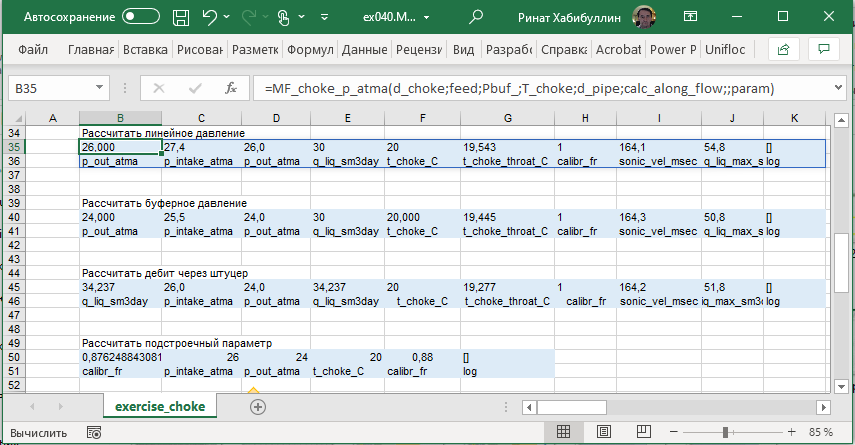
\includegraphics[width=1\linewidth]{choke_array_out}}
	\caption{Пример вывода результата расчета в массив}
	\label{ris:choke_array_out}
\end{figure}

%Функции расчёта штуцера поддерживают вычисления потока чистого газа через штуцер. Для этого в PVT строке надо установить \mintinline{vb.net}{gas_only=True} и задать расход газа параметром \mintinline{vb.net}{q_gas_sm3day} в соответствующей функции. 

\subsection{MF\_choke\_p\_atma – Расчет давления на входе или на выходе штуцера}
Функция позволяет рассчитать давление на входе или выходе штуцера по известному давлению на противоположном конце при известных параметрах потока (дебите жидкости, обводнённости, газовому фактору). Расчёт проводится по корреляции Перкинса \cite{Perkins_1993} с учётом многофазного потока. 
 
\putlisting{listings/MF_choke_p_atma.lst}

Часть настроек управляющая выводом результатов задается в виде закодированной строки в аргументе \mintinline{vb.net}{param}.

\begin{table}[H]
	\caption{Параметры функции \mintinline{vb.net}{MF_choke_p_atma} передаваемые через аргумент -- \mintinline{vb.net}{param}}
	\label{table:param_list_2}
	\begin{tabular}{p{0.2\textwidth}p{0.75\textwidth}}
		\hline
		Ключ & Описание  \\ \hline
		\mintinline{vb.net}{show_array} & Показывать расширенные результаты расчета: 0 -- результат в виде одного числа (значение по умолчанию), 1 -- результат в виде массива.    \\ \hline
		
		\mintinline{vb.net}{show_log} & Показывать лог расчета в выводе. 0 -- лог выводиться не будет, 1 -- будет показан лог в виде json строки в массиве вывода. Большой размер лога может вызвать проблемы на некоторых версиях Excel.   \\ \hline
		
		\mintinline{vb.net}{num_value} & Номер параметра выводимого на первом месте. Позволяет подменить выводимый параметр при \mintinline{vb.net}{show_array=0} на необходимый. Номера можно определить по расширенному выводу при \mintinline{vb.net}{show_array=1}  \\ \hline
		
	\end{tabular}
\end{table}

При включенной опции \mintinline{vb.net}{show_array=1} результат выдается в виде двумерного массива значений - плоской таблицы. Результирующая таблица может быть непосредственно выведена в ячейки Excel (в версиях не поддерживающие динамические массивы необходимо использовать Cntrl-Shift-Enter для вывода результата в заранее выделенный диапазон ячеек) или получена в виде массива при вызове из VBA.

При выводе массива на лист Excel первая строка содержит значения параметров, вторая подписи к значениям. При выводе с использованием Cntrl-Shift-Enter можно вывести только первую строку параметров и распространить расчетную формулу "протягиванием" на несколько строк.

\begin{table}[H]
	\caption{Расширенные результаты расчета}
	\label{table:param_list_1}
	\begin{tabular}{p{0.05\textwidth}p{0.3\textwidth}p{0.5\textwidth}}
		\hline
		№& Параметр & Описание  \\ \hline
		0 & Параметр по умолчанию & Параметр который выводится при \mintinline{vb.net}{show_array=0} или при подавлении вывода массива. Может быть настроен опцией  \mintinline{vb.net}{num_value}    \\ \hline
		
		1 & \mintinline{vb.net}{p_intake_atma} & Давление на входе в штуцер, атм    \\ \hline
		2 & \mintinline{vb.net}{p_out_atma} & Давление на выходе из штуцер, атм    \\ \hline
		3 & \mintinline{vb.net}{q_liq_sm3day} & Расход жидкости в стандартных условиях через штуцер, м$^3$/сут    \\ \hline
		4 & \mintinline{vb.net}{t_choke_C} & Температура флюида на входе и выходе из штуцера, С  \\ \hline
		5 & \mintinline{vb.net}{t_choke_throat_C} & Температура флюида внутри штуцера, в области с наибольшей скоростью, С  \\ \hline
		6 & \mintinline{vb.net}{calibr_fr} & Калибровочный параметр для модели штуцера  \\ \hline
		7 & \mintinline{vb.net}{sonic_vel_msec} & Скорость звука для флюида в проходном сечении штуцера, м/сек  \\ \hline
		8 & \mintinline{vb.net}{q_liq_max_sm3day} & Максимально возможный дебит жидкости через штуцер при заданном давлении на входе, м$^3$/сут  \\ \hline
		9 & \mintinline{vb.net}{log} & Лог расчета, выводится при \mintinline{vb.net}{show_log = 1}  \\ \hline
		
	\end{tabular}
\end{table}

При расчете предполагается, что температура флюида в штуцере не изменяется, однако в проходном сечении штуцера в корреляции Перкинса учитывается снижение температуры газа при снижении давления. Расчетное значение температуры выводится в как  \mintinline{vb.net}{t_choke_throat_C}. Также выводится скорость звука в сечении \mintinline{vb.net}{sonic_vel_msec}, которая достигается при критическом потока флюида и также выводится дебит \mintinline{vb.net}{q_liq_max_sm3day} при котором критический поток достигается. 



\subsection{MF\_choke\_q\_sm3day – функция расчёта дебита жидкости через штуцер}
Функция позволяет рассчитать по известному буферному давлению и линейному давлению дебит жидкости. Расчет  проводится по корреляции Перкинса \cite{Perkins_1993} с учетом многофазного потока.  

\putlisting{listings/MF_choke_q_sm3day.lst}

Часть настроек управляющая выводом результатов задается в виде закодированной строки в аргументе \mintinline{vb.net}{param}.

\begin{table}[H]
	\caption{Параметры функции  \mintinline{vb.net}{MF_choke_q_sm3day} передаваемые через аргумент -- \mintinline{vb.net}{param}}
	\label{table:param_list_choke_q_1}
	\begin{tabular}{p{0.2\textwidth}p{0.75\textwidth}}
		\hline
		Ключ & Описание  \\ \hline
		\mintinline{vb.net}{show_array} & Показывать расширенные результаты расчета: 0 -- результат в виде одного числа (значение по умолчанию), 1 -- результат в виде массива.    \\ \hline
		
		\mintinline{vb.net}{show_log} & Показывать лог расчета в выводе. 0 -- лог выводиться не будет, 1 -- будет показан лог в виде json строки в массиве вывода. Большой размер лога может вызвать проблемы на некоторых версиях Excel.   \\ \hline
		
		\mintinline{vb.net}{num_value} & Номер параметра выводимого на первом месте. Позволяет подменить выводимый параметр при \mintinline{vb.net}{show_array=0} на необходимый. Номера можно определить по расширенному выводу при \mintinline{vb.net}{show_array=1}  \\ \hline
		
	\end{tabular}
\end{table}

При включенной опции \mintinline{vb.net}{show_array=1} результат выдается в виде двумерного массива значений - плоской таблицы. Результирующая таблица может быть непосредственно выведена в ячейки Excel (в версиях не поддерживающие динамические массивы необходимо использовать Cntrl-Shift-Enter для вывода результата в заранее выделенный диапазон ячеек) или получена в виде массива при вызове из VBA.

При выводе массива на лист Excel первая строка содержит значения параметров, вторая подписи к значениям. При выводе с использованием Cntrl-Shift-Enter можно вывести только первую строку параметров и распространить расчетную формулу "протягиванием" на несколько строк.

\begin{table}[H]
	\caption{Расширенный вывод функции \mintinline{vb.net}{MF_choke_q_sm3day}}
	\label{table:param_list_choke_q}
	\begin{tabular}{p{0.05\textwidth}p{0.3\textwidth}p{0.5\textwidth}}
		\hline
		№& Параметр & Описание  \\ \hline
		0 & Параметр по умолчанию & Параметр который выводится при \mintinline{vb.net}{show_array=0} или при подавлении вывода массива. Может быть настроен опцией  \mintinline{vb.net}{num_value}    \\ \hline
		
		1 & \mintinline{vb.net}{p_intake_atma} & Давление на входе в штуцер, атм    \\ \hline
		2 & \mintinline{vb.net}{p_out_atma} & Давление на выходе из штуцер, атм    \\ \hline
		3 & \mintinline{vb.net}{q_liq_sm3day} & Расход жидкости в стандартных условиях через штуцер, м$^3$/сут    \\ \hline
		4 & \mintinline{vb.net}{t_choke_C} & Температура флюида на входе и выходе из штуцера, С  \\ \hline
		5 & \mintinline{vb.net}{t_choke_throat_C} & Температура флюида внутри штуцера, в области с наибольшей скоростью, С  \\ \hline
		6 & \mintinline{vb.net}{calibr_fr} & Калибровочный параметр для модели штуцера  \\ \hline
		7 & \mintinline{vb.net}{sonic_vel_msec} & Скорость звука для флюида в проходном сечении штуцера, м/сек  \\ \hline
		8 & \mintinline{vb.net}{q_liq_max_sm3day} & Максимально возможный дебит жидкости через штуцер при заданном давлении на входе, м$^3$/сут  \\ \hline
		9 & \mintinline{vb.net}{log} & Лог расчета, выводится при \mintinline{vb.net}{show_log = 1}  \\ \hline
		
	\end{tabular}
\end{table}

%Если при формировании PVT строки задать параметр \mintinline{vb.net}{gas_only=True}, то расчет будет проведен для потока газа.

\subsection{MF\_choke\_calibr\_fast – простая и быстрая функция настройки модели штуцера}
Функция позволяет рассчитать корректирующий фактор для модели штуцера, позволяющий согласовать результаты замеров давления и дебита. Расчет проводится по корреляции Перкинса \cite{Perkins_1993} с учетом многофазного потока.  

Это быстрый способ расчета калибровочного коэффициента. По факту он просто вычисляется исходя из модели штуцера.
В более сложной функции калибровки \mintinline{vb.net}{MF_calibr_choke} расчет будет проводится дольше, так как подстроечные параметры подбираются итеративным алгоритмом, зато имеется возможность подбора нескольких различных параметров.

\putlisting{listings/MF_choke_calibr_fast.lst}

%Если при формировании PVT строки задать параметр \mintinline{vb.net}{gas_only=True}, то расчет проведен не будет.
Часть настроек управляющая выводом результатов задается в виде закодированной строки в аргументе \mintinline{vb.net}{param}.

\begin{table}[H]
	\caption{Параметры функции  \mintinline{vb.net}{MF_choke_calibr_fast} передаваемые через аргумент -- \mintinline{vb.net}{param}}
	\label{table:param_list_choke_calibr_fast}
	\begin{tabular}{p{0.2\textwidth}p{0.75\textwidth}}
		\hline
		Ключ & Описание  \\ \hline
		\mintinline{vb.net}{show_array} & Показывать расширенные результаты расчета: 0 -- результат в виде одного числа (значение по умолчанию), 1 -- результат в виде массива.    \\ \hline
		
		\mintinline{vb.net}{show_log} & Показывать лог расчета в выводе. 0 -- лог выводиться не будет, 1 -- будет показан лог в виде json строки в массиве вывода. Большой размер лога может вызвать проблемы на некоторых версиях Excel.   \\ \hline
		
		\mintinline{vb.net}{num_value} & Номер параметра выводимого на первом месте. Позволяет подменить выводимый параметр при \mintinline{vb.net}{show_array=0} на необходимый. Номера можно определить по расширенному выводу при \mintinline{vb.net}{show_array=1}  \\ \hline
	\end{tabular}
\end{table}

При включенной опции \mintinline{vb.net}{show_array=1} результат выдается в виде двумерного массива значений - плоской таблицы. Результирующая таблица может быть непосредственно выведена в ячейки Excel (в версиях не поддерживающие динамические массивы необходимо использовать Cntrl-Shift-Enter для вывода результата в заранее выделенный диапазон ячеек) или получена в виде массива при вызове из VBA.

При выводе массива на лист Excel первая строка содержит значения параметров, вторая подписи к значениям. При выводе с использованием Cntrl-Shift-Enter можно вывести только первую строку параметров и распространить расчетную формулу "протягиванием" на несколько строк.

\begin{table}[H]
	\caption{Расширенный вывод функции \mintinline{vb.net}{MF_choke_calibr_fast}}
	\label{table:res_list_choke_calibr_fast}
	\begin{tabular}{p{0.05\textwidth}p{0.3\textwidth}p{0.5\textwidth}}
		\hline
		№& Параметр & Описание  \\ \hline
		0 & \mintinline{vb.net}{calibr_fr} & Параметр калибровки или другой параметр в зависимости от значения опции 	\mintinline{vb.net}{num_value}     \\ \hline
		
		1 & \mintinline{vb.net}{p_intake_atma} & Давление на входе в штуцер, атм    \\ \hline
		2 & \mintinline{vb.net}{p_out_atma} & Давление на выходе из штуцер, атм    \\ \hline
		3 & \mintinline{vb.net}{t_choke_C} & Температура флюида на входе и выходе из штуцера, С  \\ \hline
		
		4 & \mintinline{vb.net}{calibr_fr} & Параметр калибровки    \\ \hline
		
		5 & \mintinline{vb.net}{log} & Лог расчета, выводится при \mintinline{vb.net}{show_log = 1}  \\ \hline
		
	\end{tabular}
\end{table}

\subsection{MF\_choke\_calc – расчет штуцера с полным выводом}
Функция позволяет рассчитать давление на выходе или входе штуцера, аналогично функции \mintinline{vb.net}{MF_choke_p_atma}. Но в отличии от нее выдает результаты в виде нескольких json строк скомпонованных в двумерный массив. Такой подход более универсален и легче расширяется, легче переносится в другие языки программирования, но при работе с Excel может вызывать проблемы с некоторыми версиями Excel (вывод длинных строк при выводе массива может некорректно работать в Excel 2016).

В функцию заложена следующая логика работы -- поток, включая дебит должен быть задан. При одном заданном давлении на входе или на выходе второе будет рассчитанно с заданным потоком. При двух заданных давлениях -- будет рассчитан дебит жидкости и скорректированы параметры потока.

Расчёт проводится по корреляции Перкинса \cite{Perkins_1993} с учётом многофазного потока. 

\putlisting{listings/MF_choke_calc.lst}

Часть настроек управляющая выводом результатов задается в виде закодированной строки в аргументе \mintinline{vb.net}{param}.

\begin{table}[H]
	\caption{Параметры функции \mintinline{vb.net}{MF_choke_calc} передаваемые через аргумент -- \mintinline{vb.net}{param}}
	\label{table:param_list_3}
	\begin{tabular}{p{0.2\textwidth}p{0.75\textwidth}}
		\hline
		Ключ & Описание  \\ \hline
		\mintinline{vb.net}{show_array} & Показывать расширенные результаты расчета: 0 -- результат в виде одного числа (значение по умолчанию), 1 -- результат в виде массива.    \\ \hline
		
		\mintinline{vb.net}{show_log} & Показывать лог расчета в выводе. 0 -- лог выводиться не будет, 1 -- будет показан лог в виде json строки в массиве вывода. Большой размер лога может вызвать проблемы на некоторых версиях Excel.   \\ \hline
		
		
	\end{tabular}
\end{table}
 
При включенной опции \mintinline{vb.net}{show_array=1} результат выдается в виде двумерного массива значений - плоской таблицы. Результирующая таблица может быть непосредственно выведена в ячейки Excel (в версиях не поддерживающие динамические массивы необходимо использовать Cntrl-Shift-Enter для вывода результата в заранее выделенный диапазон ячеек) или получена в виде массива при вызове из VBA.
 
При выводе массива на лист Excel первая строка содержит значения параметров, вторая подписи к значениям. При выводе с использованием Cntrl-Shift-Enter можно вывести только первую строку параметров и распространить расчетную формулу "протягиванием" на несколько строк.
 
\begin{table}[H]
	\caption{Расширенный вывод функции \mintinline{vb.net}{MF_choke_calc} }
	\label{table:param_list_MF_choke_calc}
	\begin{tabular}{p{0.05\textwidth}p{0.3\textwidth}p{0.5\textwidth}}
		\hline
		№& Параметр & Описание  \\ \hline
		0 & \mintinline{vb.net}{json} & json строка с результатами расчета  \\ \hline
		
		1 & \mintinline{vb.net}{feed} & Параметры потока использованные для расчета в виде json строки\\ \hline
		2 & \mintinline{vb.net}{log} & Лог расчета, выводится при \mintinline{vb.net}{show_log = 1}  \\ \hline
		
	\end{tabular}
\end{table}
 
\begin{table}[H]
	\caption{json строка с результатами расчета функции \mintinline{vb.net}{MF_choke_calc} }
	\label{table:param_list_choke_calc}
	\begin{tabular}{p{0.05\textwidth}p{0.3\textwidth}p{0.5\textwidth}}
		\hline
		№& Параметр & Описание  \\ \hline
		
		1 & \mintinline{vb.net}{p_intake_atma} & Давление на входе в штуцер, атм    \\ \hline
		2 & \mintinline{vb.net}{p_out_atma} & Давление на выходе из штуцер, атм    \\ \hline
		3 & \mintinline{vb.net}{t_choke_C} & Температура флюида на входе и выходе из штуцера, С  \\ \hline
		4 & \mintinline{vb.net}{calibr_fr} & Калибровочный параметр для модели штуцера  \\ \hline
		5 & \mintinline{vb.net}{q_liq_sm3day} & Расход жидкости в стандартных условиях через штуцер, м$^3$/сут    \\ \hline
		6 & \mintinline{vb.net}{q_gas_sm3day} & Расход газа в стандартных условиях через штуцер, м$^3$/сут    \\ \hline
		7 & \mintinline{vb.net}{q_gas_free_sm3day} & Расход свободного газа (дополнительного к растворенному) в стандартных условиях через штуцер, м$^3$/сут    \\ \hline
		8 & \mintinline{vb.net}{rp_m3m3} &  Газовый фактор потока  \\ \hline
		9 & \mintinline{vb.net}{fw_perc} &  Обводненность потока, в процентах \\ \hline
		10 & \mintinline{vb.net}{t_choke_throat_C} & Температура флюида внутри штуцера, в области с наибольшей скоростью, С  \\ \hline
		11 & \mintinline{vb.net}{sonic_vel_msec} & Скорость звука для флюида в проходном сечении штуцера, м/сек  \\ \hline
		12 & \mintinline{vb.net}{q_liq_max_sm3day} & Максимально возможный дебит жидкости через штуцер при заданном давлении на входе, м$^3$/сут  \\ \hline
		
	\end{tabular}
\end{table}
 
 При расчете предполагается, что температура флюида в штуцере не изменяется, однако в проходном сечении штуцера в корреляции Перкинса учитывается снижение температуры газа при снижении давления. Расчетное значение температуры выводится в как  \mintinline{vb.net}{t_choke_throat_C}. Также выводится скорость звука в сечении \mintinline{vb.net}{sonic_vel_msec}, которая достигается при критическом потока флюида и также выводится дебит \mintinline{vb.net}{q_liq_max_sm3day} при котором критический поток достигается. 
 
 

\subsection{MF\_choke\_calibr – продвинутая функция настройки модели штуцера}
Функция позволяет рассчитать корректирующий фактор для модели штуцера, позволяющий согласовать результаты замеров давления и дебита. Расчет проводится по корреляции Перкинса \cite{Perkins_1993} с учетом многофазного потока.  

Настройка может проводиться за счет подбора различных параметров. Тип калибровки выбирается параметром \mintinline{vb.net}{calibr_type}. В текущей реализации может быть подобран только один из перечисленных ниже параметров.

\begin{itemize}
	\item \mintinline{vb.net}{calibr_type=0} Калибровочный коэффициент многофазной корреляции для гравитационной составляющей  $c_{calibr\_grav}$. Ищется в диапазоне от 0.5 до 1.5.
	\item \mintinline{vb.net}{calibr_type=1} Калибровочный коэффициент многофазной корреляции для трения $c_{calibr\_fric}$. Ищется в диапазоне от 0.5 до 1.5.
	\item \mintinline{vb.net}{calibr_type=2} Газовый фактор $R_p$. Ищется в диапазоне $[20, 2 R_p]$ относительно заданного газового фактора. 
	\item \mintinline{vb.net}{calibr_type=3} Обводненность $f_w$.  Значение ищется в диапазоне $[0, 1]$.  
	\item \mintinline{vb.net}{calibr_type=4} Дебит жидкости \(Q_{liq}\). Значение ищется в диапазоне от \([0.. Q_{liq} \cdot 1.5]\) относительно заданного дебита жидкости. 	 
	\item \mintinline{vb.net}{calibr_type=5} Дебит газа \(Q_{gas}\). Значение ищется  в диапазоне от \([0.. Q_{gas} \cdot 2]\) относительно заданного дебита газа или в диапазоне \([0..10000]\) м$^3$/сут если дебит газа не задан. 	
\end{itemize}

Результат расчета - массив с подобранным параметром или сообщением о невозможности подбора, информацией о количестве итераций. 

\putlisting{listings/MF_choke_calibr.lst}

Часть настроек управляющая выводом результатов задается в виде закодированной строки в аргументе \mintinline{vb.net}{param}.

\begin{table}[H]
	\caption{Параметры функции  \mintinline{vb.net}{MF_choke_calibr} передаваемые через аргумент -- \mintinline{vb.net}{param}}
	\label{table:param_list_choke_calibr}
	\begin{tabular}{p{0.2\textwidth}p{0.75\textwidth}}
		\hline
		Ключ & Описание  \\ \hline
		\mintinline{vb.net}{show_array} & Показывать расширенные результаты расчета: 0 -- результат в виде одного числа (значение по умолчанию), 1 -- результат в виде массива.    \\ \hline
		
		\mintinline{vb.net}{show_log} & Показывать лог расчета в выводе. 0 -- лог выводиться не будет, 1 -- будет показан лог в виде json строки в массиве вывода. Большой размер лога может вызвать проблемы на некоторых версиях Excel.   \\ \hline
		
	\end{tabular}
\end{table}

При включенной опции \mintinline{vb.net}{show_array=1} результат выдается в виде двумерного массива значений - плоской таблицы. Результирующая таблица может быть непосредственно выведена в ячейки Excel (в версиях не поддерживающие динамические массивы необходимо использовать Cntrl-Shift-Enter для вывода результата в заранее выделенный диапазон ячеек) или получена в виде массива при вызове из VBA.

При выводе массива на лист Excel первая строка содержит значения параметров, вторая подписи к значениям. При выводе с использованием Cntrl-Shift-Enter можно вывести только первую строку параметров и распространить расчетную формулу "протягиванием" на несколько строк.

\begin{table}[H]
	\caption{Расширенный вывод функции \mintinline{vb.net}{MF_choke_calibr} }
	\label{table:param_list_MF_choke_calibr}
	\begin{tabular}{p{0.05\textwidth}p{0.3\textwidth}p{0.5\textwidth}}
		\hline
		№& Параметр & Описание  \\ \hline
		0 & \mintinline{vb.net}{result} & json строка с результатами расчета подстраиваемого параметра \\ \hline
		1 & \mintinline{vb.net}{last calc} & json строка с результатами расчета параметров штуцера для подобранного параметра \\ \hline
		2 & \mintinline{vb.net}{feed} & Параметры потока использованные для расчета в виде json строки\\ \hline
		3 & \mintinline{vb.net}{log} & Лог расчета, выводится при \mintinline{vb.net}{show_log = 1}  \\ \hline
		
	\end{tabular}
\end{table}

\begin{table}[H]
	\caption{json строка с результатами расчета функции \mintinline{vb.net}{MF_choke_calc} }
	\label{table:param_list_MF_choke_calc_json}
	\begin{tabular}{p{0.05\textwidth}p{0.3\textwidth}p{0.5\textwidth}}
		\hline
		№& Параметр & Описание  \\ \hline
		
		1 & \mintinline{vb.net}{p_intake_atma} & Давление на входе в штуцер, атм    \\ \hline
		2 & \mintinline{vb.net}{p_out_atma} & Давление на выходе из штуцер, атм    \\ \hline
		3 & \mintinline{vb.net}{t_choke_C} & Температура флюида на входе и выходе из штуцера, С  \\ \hline
		4 & \mintinline{vb.net}{calibr_fr} & Калибровочный параметр для модели штуцера  \\ \hline
		5 & \mintinline{vb.net}{q_liq_sm3day} & Расход жидкости в стандартных условиях через штуцер, м$^3$/сут    \\ \hline
		6 & \mintinline{vb.net}{q_gas_sm3day} & Расход газа в стандартных условиях через штуцер, м$^3$/сут    \\ \hline
		7 & \mintinline{vb.net}{q_gas_free_sm3day} & Расход свободного газа (дополнительного к растворенному) в стандартных условиях через штуцер, м$^3$/сут    \\ \hline
		8 & \mintinline{vb.net}{rp_m3m3} &  Газовый фактор потока  \\ \hline
		9 & \mintinline{vb.net}{fw_perc} &  Обводненность потока, в процентах \\ \hline
		10 & \mintinline{vb.net}{t_choke_throat_C} & Температура флюида внутри штуцера, в области с наибольшей скоростью, С  \\ \hline
		11 & \mintinline{vb.net}{sonic_vel_msec} & Скорость звука для флюида в проходном сечении штуцера, м/сек  \\ \hline
		12 & \mintinline{vb.net}{q_liq_max_sm3day} & Максимально возможный дебит жидкости через штуцер при заданном давлении на входе, м$^3$/сут  \\ \hline
		
	\end{tabular}
\end{table}

\newpage
\section{Расчет многофазного потока в трубе}

Для расчёта участка трубы с использованием пользовательских функций \unf{} применяется схема показанная на рисунке \ref{ris:Pipe_scheme_1}. Труба задается набором значений измеренной $[L_0, L_1,..,L_n]$ и вертикальных $[H_{vn}, H_{vn},..,H_{vn}]$ глубин, описывающих траекторию и набором значений измеренной глубины $[L_0, L_1,..,L_k]$ и диаметров $[d_0, d_1,..,d_k]$. Для каждой точки трубы значения угла наклона и диаметра этого участка определяется линейной интерполяцией соответствующих массивов. Для формирования данных в виде json строки можно использовать функцию  \mintinline{vb.net}{encode_pipe}.

\begin{figure}[H]
	\begin{center}
		

\tikzset{every picture/.style={line width=0.75pt}} %set default line width to 0.75pt        

\begin{tikzpicture}[x=0.75pt,y=0.75pt,yscale=-1,xscale=1]
%uncomment if require: \path (0,368); %set diagram left start at 0, and has height of 368

%Shape: Can [id:dp6216173981316635] 
\draw  [fill={rgb, 255:red, 250; green, 245; blue, 184 }  ,fill opacity=1 ][line width=1.5]  (366.75,232.82) -- (522.77,233.82) .. controls (524.76,233.84) and (526.34,239.22) .. (526.3,245.85) .. controls (526.25,252.47) and (524.61,257.84) .. (522.62,257.82) -- (366.59,256.82) .. controls (364.61,256.8) and (363.03,251.42) .. (363.07,244.79) .. controls (363.12,238.17) and (364.76,232.8) .. (366.75,232.82) .. controls (368.74,232.83) and (370.31,238.21) .. (370.27,244.84) .. controls (370.23,251.47) and (368.58,256.83) .. (366.59,256.82) ;
%Shape: Can [id:dp907638736363561] 
\draw  [fill={rgb, 255:red, 250; green, 245; blue, 184 }  ,fill opacity=1 ][line width=1.5]  (240.84,162.19) -- (379.01,233.11) .. controls (380.96,234.11) and (379.83,240.18) .. (376.51,246.66) .. controls (373.18,253.15) and (368.9,257.59) .. (366.96,256.6) -- (228.79,185.68) .. controls (226.84,184.68) and (227.96,178.61) .. (231.29,172.13) .. controls (234.62,165.64) and (238.9,161.19) .. (240.84,162.19) .. controls (242.79,163.19) and (241.67,169.26) .. (238.34,175.74) .. controls (235.01,182.23) and (230.73,186.68) .. (228.79,185.68) ;
%Shape: Can [id:dp8065516167465729] 
\draw  [fill={rgb, 255:red, 250; green, 245; blue, 184 }  ,fill opacity=1 ][line width=1.5]  (162.57,41.83) -- (252.52,167.06) .. controls (253.98,169.09) and (249.68,174.67) .. (242.92,179.52) .. controls (236.16,184.38) and (229.5,186.67) .. (228.04,184.64) -- (138.09,59.42) .. controls (136.64,57.39) and (140.94,51.81) .. (147.7,46.95) .. controls (154.46,42.1) and (161.12,39.8) .. (162.57,41.83) .. controls (164.03,43.86) and (159.73,49.44) .. (152.97,54.3) .. controls (146.21,59.15) and (139.55,61.44) .. (138.09,59.42) ;
%Straight Lines [id:da4209568517236453] 
\draw    (542.3,44.83) -- (542.3,176.52) ;
\draw [shift={(542.3,179.52)}, rotate = 270] [fill={rgb, 255:red, 0; green, 0; blue, 0 }  ][line width=0.08]  [draw opacity=0] (8.93,-4.29) -- (0,0) -- (8.93,4.29) -- cycle    ;
\draw [shift={(542.3,41.83)}, rotate = 90] [fill={rgb, 255:red, 0; green, 0; blue, 0 }  ][line width=0.08]  [draw opacity=0] (8.93,-4.29) -- (0,0) -- (8.93,4.29) -- cycle    ;
%Straight Lines [id:da44510371664546344] 
\draw    (542.3,181.47) -- (542.3,241.79) ;
\draw [shift={(542.3,244.79)}, rotate = 270] [fill={rgb, 255:red, 0; green, 0; blue, 0 }  ][line width=0.08]  [draw opacity=0] (8.93,-4.29) -- (0,0) -- (8.93,4.29) -- cycle    ;
\draw [shift={(542.3,178.47)}, rotate = 90] [fill={rgb, 255:red, 0; green, 0; blue, 0 }  ][line width=0.08]  [draw opacity=0] (8.93,-4.29) -- (0,0) -- (8.93,4.29) -- cycle    ;
%Straight Lines [id:da9486867990230097] 
\draw    (130.42,74.5) -- (161.37,113.98) ;
\draw [shift={(162.6,115.55)}, rotate = 231.91] [color={rgb, 255:red, 0; green, 0; blue, 0 }  ][line width=0.75]    (10.93,-3.29) .. controls (6.95,-1.4) and (3.31,-0.3) .. (0,0) .. controls (3.31,0.3) and (6.95,1.4) .. (10.93,3.29)   ;
%Straight Lines [id:da43751816745520045] 
\draw  [dash pattern={on 4.5pt off 4.5pt}]  (162.57,41.83) -- (557.37,41.83) ;
%Straight Lines [id:da3288286521166641] 
\draw  [dash pattern={on 4.5pt off 4.5pt}]  (242.92,179.52) -- (554.3,179.52) ;
%Straight Lines [id:da5448798037206697] 
\draw  [dash pattern={on 4.5pt off 4.5pt}]  (526.3,244.84) -- (548.8,244.84) ;

% Text Node
\draw (221.92,189.9) node [anchor=north west][inner sep=0.75pt]    {$L_{1}$};
% Text Node
\draw (368.96,260) node [anchor=north west][inner sep=0.75pt]    {$L_{2}$};
% Text Node
\draw (511.6,259.9) node [anchor=north west][inner sep=0.75pt]    {$L_{3}$};
% Text Node
\draw (552.6,158.92) node [anchor=north west][inner sep=0.75pt]    {$H_{v}{}_{1}$};
% Text Node
\draw (552.6,236.74) node [anchor=north west][inner sep=0.75pt]    {$H_{v}{}_{2}$};
% Text Node
\draw (585.1,236.74) node [anchor=north west][inner sep=0.75pt]    {$H_{v}{}_{3}$};
% Text Node
\draw (125.69,79.28) node [anchor=north west][inner sep=0.75pt]  [rotate=-52.7]  {$coord$};
% Text Node
\draw (169.6,26.35) node [anchor=north west][inner sep=0.75pt]    {$P_{1}$};
% Text Node
\draw (516.8,213.85) node [anchor=north west][inner sep=0.75pt]    {$P_{2}$};
% Text Node
\draw (116.92,51.9) node [anchor=north west][inner sep=0.75pt]    {$L_{0}$};
% Text Node
\draw (552.6,31.92) node [anchor=north west][inner sep=0.75pt]    {$H_{v}{}_{0}$};


\end{tikzpicture}
		\caption{Схема трубы принятая для расчётов с использованием пользовательских функций}
		\label{ris:Pipe_scheme_1}
	\end{center}
\end{figure}

Координата трубы возрастает от начала к концу (исходные массивы всегда будут автоматически сортироваться). Относительно направления координаты задаются направление расчета и направление потока соответствующими параметрами расчетных функций \mintinline{vb.net}{calc_along_coord} и \mintinline{vb.net}{flow_along_coord}

Труба имеет постоянную по всей длине шероховатость стенок. Шероховатость влияет на коэффициент трения при расчете потока и проявляется при относительно больших скоростях потока. Подробнее про шероховатость и трение в потоке жидкости можно почитать в \cite{Bratland_Pipe_Flow_1}

\subsection{Задание конструкции трубы \mintinline{vb.net}{encode_pipe}}

Детальная конструкция трубы включая траекторию и диаметры может быть сформирована в виде json строки с использованием функции \mintinline{vb.net}{encode_pipe}.

\putlisting{listings/encode_pipe.lst}


\subsection{Задание температурных параметров для расчета трубы \mintinline{vb.net}{encode_t_model}}

Расчет трубы может быть проведен с использованием нескольких температурных моделей, выбор которых определяется опцией \mintinline{vb.net}{t_model}  набора параметров температурной модели задаваемых json строкой, которую можно сгенерировать функцией \mintinline{vb.net}{encode_t_model}

\putlisting{listings/encode_t_model.lst}

доступные модели 

\begin{table}[H]
	\caption{Доступные модели расчета температуры}
	\label{table:model_list_t_model}
	\begin{tabular}{p{0.05\textwidth}p{0.2\textwidth}p{0.65\textwidth}}
		\hline
		№& Параметр & Описание  \\ \hline
		
		1 & \mintinline{vb.net}{t_model = 0} & Значение по умолчанию. Температура линейно меняется по длине трубы, задается значениями температуры на концах трубы, опции \mintinline{vb.net}{t_start_C} и \mintinline{vb.net}{t_end_C}   \\ \hline
		2 & \mintinline{vb.net}{t_model = 1} & Температура флюида равна заданной температуре окружающей среды. Температура окружающей среды задается опцией \mintinline{vb.net}{t_list_C}    \\ \hline
		3 & \mintinline{vb.net}{t_model = 2} &Температура флюида рассчитывается с учетом  заданной температуры окружающей среды и теплопотерь. Температура окружающей среды задается опцией \mintinline{vb.net}{t_list_C}. Параметры теплопередачи задаются соответствующими опциями   \\ \hline
		4 & \mintinline{vb.net}{t_model = 3} &Температура флюида равна заданной температуре относительно измеренной глубины.Заданная температура задается опцией \mintinline{vb.net}{t_list_C}     \\ \hline
		
	\end{tabular}
\end{table}

Значения опций закодированных в json строке меняются в зависимости от выбранной модели. Часть опций можно задать с использованием аргумента функции \mintinline{vb.net}{param}.

Опции для \mintinline{vb.net}{t_model = 2} приведены в таблице ниже. Расчетная модель реализована на основе работы \cite{HasanKabir_HeatTransfer_2002}.

\begin{table}[H]
	\caption{Параметры функции  \mintinline{vb.net}{encode_t_model} передаваемые через аргумент -- \mintinline{vb.net}{param}}
	\label{table:param_list_t_model_param}
	\begin{tabular}{p{0.63\textwidth}p{0.32\textwidth}}
		\hline
		Ключ & Описание  \\ \hline
		\mintinline{vb.net}{thermal_conductivity_formation_WmC} & Теплопроводность пласта   \\ \hline
		
		\mintinline{vb.net}{specific_heat_capacity_formation_JkgC} & Теплоемкость пласта   \\ \hline
		
		\mintinline{vb.net}{thermal_conductivity_cement_WmC} & Теплопроводность цемента вокруг скважины\\ \hline
		
		\mintinline{vb.net}{thermal_conductivity_tubing_WmC} & Теплопроводность НКТ\\ \hline
		
		\mintinline{vb.net}{thermal_conductivity_casing_WmC} & Теплопроводность эксплуатационной колонны\\ \hline
		
		\mintinline{vb.net}{heat_transfer_casing_liquid_Wm2C} & Температуропроводность межтрубного пространства с жидкостью\\ \hline
		
		\mintinline{vb.net}{heat_transfer_casing_gas_Wm2C} & Температуропроводность межтрубного пространства с газом\\ \hline
		
		\mintinline{vb.net}{heat_transfer_fluid_convection_Wm2C} & Температуропроводность флюида в НКТ за счет конвекции\\ \hline
		
		\mintinline{vb.net}{time_calc_hr} & Время расчета\\ \hline
	\end{tabular}
\end{table}

Значения по умолчанию для приведенных величин можно узнать запустив функцию \mintinline{vb.net}{encode_t_model} без параметров и расшифровав ее результаты функцией \mintinline{vb.net}{dencode_json}. Размерности опций указаны в их названиях.  Для расчета трубы, при положительной измеренной глубине расчет реализуется для потока по эксплуатационной колонне, влияние НКТ и межтрубного пространства не учитывается.

\subsection{Задание многофазной корреляции для расчета распределения давления}

Расчет распределения давления в трубе основан на многофазных корреляциях. Выбор типа корреляции определяется параметром  \mintinline{vb.net}{flow_correlation}. В текущей версии \unf{} реализован следующий набор гидравлических корреляций:
\begin{enumerate}
	\item \mintinline{vb.net}{flow_correlation = 0}. Корреляция Беггса Брилла \cite{Mukerji_Brill_Multiphase_2006}.
	\item \mintinline{vb.net}{flow_correlation = 1}. Корреляция Ансари \cite{Mukerji_Brill_Multiphase_2006}.
	\item \mintinline{vb.net}{flow_correlation = 2}. Корреляция TUFFP Unified \cite{Khasanov_Unified_SPE_2006, Guk_Unified_2009}.
	\item \mintinline{vb.net}{flow_correlation = 3}. Корреляция Грея, модифицированная \cite{Mukerji_Brill_Multiphase_2006}.
	\item \mintinline{vb.net}{flow_correlation = 4}. Корреляция Хайгедорна Брауна \cite{Mukerji_Brill_Multiphase_2006}.
	\item \mintinline{vb.net}{flow_correlation = 5}. Корреляция Сахарова Мохова \cite{Sakharov_Mokhov_2008}.
	\item \mintinline{vb.net}{flow_correlation = 10}. Расчет на основе плотности газа, без учета жидкости.
	
\end{enumerate}

Ниже на рисунке \ref{ris:VLP_curves} приведены результаты расчёта кривой оттока (перепада давления в вертикальной трубе) для различных корреляций, реализованных в \unf{}.

\begin{figure}[H]
	\begin{center}
	\newcommand{\dPipeDataFile}{data/dPipe.txt}
		\begin{tikzpicture}[scale=1]
		\begin{axis}[
					width=14cm,
					height=10cm,
					xlabel=$Q\; m^3 / day$,
					ylabel=$P_{wf} \; atma$,
					legend pos=south east,
					title=Pipe Pressure Drop]
		\addplot table [y=P_0, x=Q]{\dPipeDataFile};
		\addlegendentry{Beggs Brill}
		\addplot table [y=P_1, x=Q]{\dPipeDataFile};
		\addlegendentry{Ansari}
		\addplot table [y=P_2, x=Q]{\dPipeDataFile};
		\addlegendentry{Unified}
		\addplot table [y=P_3, x=Q]{\dPipeDataFile};
		\addlegendentry{Gray}
		\addplot table [y=P_4, x=Q]{\dPipeDataFile};
		\addlegendentry{Hagedorn Brown}
		\addplot table [y=P_5, x=Q]{\dPipeDataFile};
		\addlegendentry{Sakharov Mokhov}
		\end{axis}
		\end{tikzpicture}	
	\caption{Кривые характеристики многофазного потока для вертикальных труб рассчитанные с использованием различных корреляций }
	\label{ris:VLP_curves}
	\end{center}
\end{figure}


\subsection{MF\_pipe\_p\_atma – функция расчета распределения давления в трубе}  


Функция позволяет рассчитать перепад давления в участке трубопровода. Функция обеспечивает несколько режимов расчёта. Некоторые особенности работы функции \mintinline{vb.net}{MF_p_pipe_atma()}
\begin{itemize}
	\item Свойства флюида в трубе определяются параметром \mintinline{vb.net}{feed}, который в свою очередь может быть задан функцией \mintinline{vb.net}{encode_feed()}.
	\item Если параметр дебита жидкости  \mintinline{vb.net}{qliq_sm3day = 0}  равен нулю, расчет проводится для режима барботажа (ZNLF - zero net liquid flow) - движения газа через неподвижный столб жидкости. Расход газа должен быть задан опцией потока \mintinline{vb.net}{q_gas_free_sm3day}. В текущей версии \unf{} расчет барботажа проводится проводится за счет переключения на механистическую корреляцию Ансари. Попытка построить график зависимости перепад давления от дебита для других корреляций может дать нелогичный результат около нулевого дебита (скачек перепада давления). Рекомендуется без необходимости для \mintinline{vb.net}{qliq_sm3day = 0} не считать при построении графиков.
	\item Распределение температуры для функции расчета участка скважины определяется температурной моделью \mintinline{vb.net}{t_model} 
\end{itemize}

\putlisting{listings/MF_pipe_p_atma.lst}

Часть настроек управляющая выводом результатов задается в виде закодированной строки в аргументе \mintinline{vb.net}{param}.

\begin{table}[H]
	\caption{Параметры функции \mintinline{vb.net}{MF_pipe_p_atma} передаваемые через аргумент -- \mintinline{vb.net}{param}}
	\label{table:param_list_pipe}
	\begin{tabular}{p{0.2\textwidth}p{0.75\textwidth}}
		\hline
		Ключ & Описание  \\ \hline
		\mintinline{vb.net}{show_array} & Показывать расширенные результаты расчета: 0 -- результат в виде одного числа (значение по умолчанию), 1 -- результат в виде массива.    \\ \hline
		
		\mintinline{vb.net}{show_log} & Показывать лог расчета в выводе. 0 -- лог выводиться не будет, 1 -- будет показан лог в виде json строки в массиве вывода. Большой размер лога может вызвать проблемы на некоторых версиях Excel.   \\ \hline
		
		\mintinline{vb.net}{num_value} & Номер параметра выводимого на первом месте. Позволяет подменить выводимый параметр при \mintinline{vb.net}{show_array=0} на необходимый. Номера можно определить по расширенному выводу при \mintinline{vb.net}{show_array=1}  \\ \hline
		
	\end{tabular}
\end{table}

При включенной опции \mintinline{vb.net}{show_array=1} результат выдается в виде двумерного массива значений - плоской таблицы. Результирующая таблица может быть непосредственно выведена в ячейки Excel (в версиях не поддерживающие динамические массивы необходимо использовать Cntrl-Shift-Enter для вывода результата в заранее выделенный диапазон ячеек) или получена в виде массива при вызове из VBA.

При выводе массива на лист Excel первая строка содержит значения параметров, вторая подписи к значениям. При выводе с использованием Cntrl-Shift-Enter можно вывести только первую строку параметров и распространить расчетную формулу "протягиванием" на несколько строк.

\begin{table}[H]
	\caption{Расширенный вывод функции \mintinline{vb.net}{MF_pipe_p_atma} }
	\label{table:res_list_pipe}
	\begin{tabular}{p{0.05\textwidth}p{0.25\textwidth}p{0.65\textwidth}}
		\hline
		№& Параметр & Описание  \\ \hline
		0 & \mintinline{vb.net}{p_result_atma} & Параметр который выводится при \mintinline{vb.net}{show_array=0} или при подавлении вывода массива. Может быть настроен опцией  \mintinline{vb.net}{num_value}. По умолчанию расчетное давление на конце трубы    \\ \hline
		
		1 & \mintinline{vb.net}{p_1, atma} & Давление на начальном конце трубы (меньшая координата по длине), атм    \\ \hline
		2 & \mintinline{vb.net}{t_1, C} &   Температура на начальном конце трубы (меньшая координата по длине), С    \\ \hline
		3 & \mintinline{vb.net}{p_2, atma} & Давление на конечном конце трубы (большая координата по длине), атм     \\ \hline
		4 & \mintinline{vb.net}{t_2, C} & Температура на конечном конце трубы (большая координата по длине), С     \\ \hline
		5 & \mintinline{vb.net}{calibr_grav} & Калибровочный коэффициент на гравитационную составляющую перепада давления   \\ \hline
		6 & \mintinline{vb.net}{calibr_fric} &  Калибровочный коэффициент на составляющую перепада давления по трению  \\ \hline
		7 & \mintinline{vb.net}{log} & Лог расчета, выводится при \mintinline{vb.net}{show_log = 1}  \\ \hline
			
	\end{tabular}
\end{table}

Векторные результаты перечисленные ниже могут быть использованы для построения графиков и для проверки корректности расчета.

\begin{table}[H]
	\caption{Расширенный вывод функции \mintinline{vb.net}{MF_pipe_p_atma}. Векторные результаты}
	\label{table:res_list_pipe_crv}
	\begin{tabular}{p{0.05\textwidth}p{0.25\textwidth}p{0.55\textwidth}}
		1 & \mintinline{vb.net}{h,m} & Вектор измеренных глубин, м   \\ \hline
		
		2 & \mintinline{vb.net}{hvert,m} & Вектор вертикальных глубин, соответствующих измеренным, м   \\ \hline
		3 & \mintinline{vb.net}{p,atma} & Вектор давлений, соответствующих измеренным глубинам, атм   \\ \hline
		4 & \mintinline{vb.net}{t,C} & Вектор температур флюида, соответствующих измеренным глубинам, С   \\ \hline
		5 & \mintinline{vb.net}{t_amb, C} & Вектор температур окружающей среды, соответствующих измеренным глубинам, С   \\ \hline
		6 & \mintinline{vb.net}{Hl, perc} & Вектор истинных содержаний жидкости (liquid holdup), соответствующих измеренным глубинам, \%   \\ \hline
		7 & \mintinline{vb.net}{fpat} & Вектор индикаторов режимов потока, соответствующих измеренным глубинам, число   \\ \hline
		8 & \mintinline{vb.net}{diam, mm} & Вектор внутренних диаметров трубы, соответствующих измеренным глубинам, мм \\ \hline
		
	\end{tabular}
\end{table}

Режимы потока для механистических корреляций кодируются по следующей схеме при проведении расчетов 
\begin{table}[H]
	\caption{Кодировка режимов потока в функции \mintinline{vb.net}{MF_pipe_p_atma}. }
	\label{table:res_list_pipe_fpat}
	\begin{tabular}{p{0.6\textwidth}p{0.15\textwidth}p{0.15\textwidth}}
		
		Режим & Ансари & TUFFP\\ \hline
		liq, жидкость & 100 & 200\\ \hline
		gas, чистый газ & 101 & 201\\ \hline
		bubl, пузырьковый & 102 & 202\\ \hline
		slug, снарядный & 103 & 205\\ \hline
		dbub, распределенный пузырьковый & 104 & 206\\ \hline
		anul, кольцевой & 105 & 207\\ \hline
		int, перемежающийся & - & 203\\ \hline
		str, разделенный & - & 204\\ \hline
		na, не определен & 199 & 299\\ \hline
		
		
	\end{tabular}
\end{table}




\subsection{MF\_dpdl\_atmm – функция расчета градиента давления по многофазной корреляции Ансари}  
Иногда бывает удобно/интересно посмотреть детально на результаты расчета по многофазной корреляции. Для этого можно воспользоваться данной функцией. Внимательно смотрите описание и саму функцию. Выводит ряд параметров в массиве.

\putlisting{listings/MF_dpdl_atmm.lst}


\begin{comment}

Результатом работы функции является массив, содержащий давления и температуру на концах трубы, калибровочные параметры, а также значения ряда параметров между концами трубы. Вывод значений между концами трубы может быть отключен установкой \mintinline{vb.net}{out_curves=False}. При необходимости проведения массовых расчетов можно вывести только одно значение (или одну строку значений) штатными средствами Excel. 

\begin{figure}[ht]
	\center{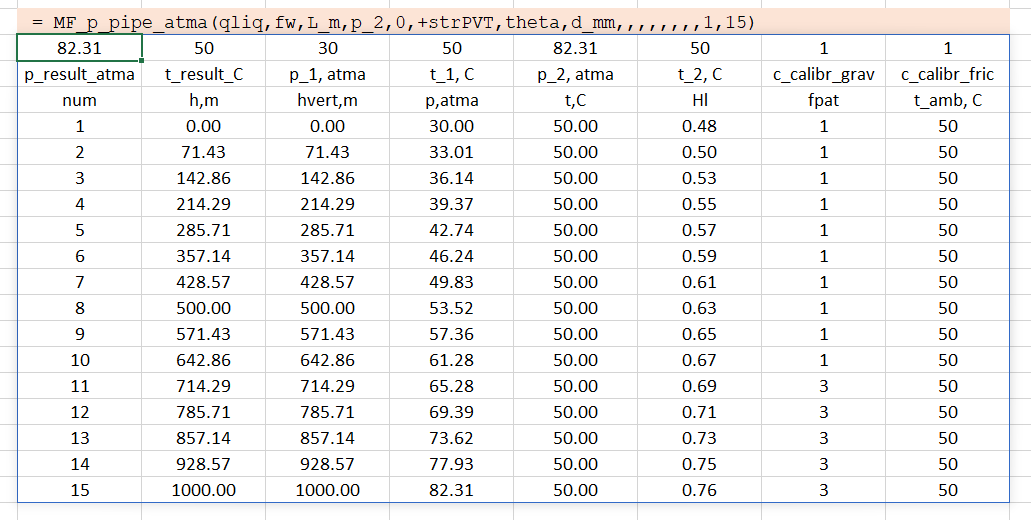
\includegraphics[width=1\linewidth]{pipe_out_example}}
	\caption{Пример вывода результатов расчета функции \mintinline{vb.net}{MF_p_pipe_atma()} для  \mintinline{vb.net}{out_curves=True} }
	\label{ris:pipe_out_example}
\end{figure}

\begin{figure}[ht]
	\center{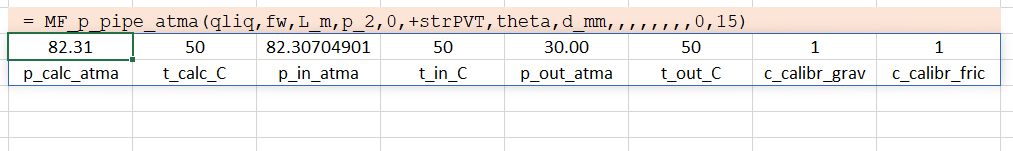
\includegraphics[width=1\linewidth]{pipe_out_example_short}}
	\caption{Пример вывода результатов расчета функции \mintinline{vb.net}{MF_p_pipe_atma()} для  \mintinline{vb.net}{out_curves=False} }
	\label{ris:pipe_out_example_short}
\end{figure}

\subsection{MF\_calibr\_pipe, MF\_calibr\_pipeline - функция калибровки расчета участка трубы}

Функция калибровки позволяет настроить модель потока в трубе под замеры давления на концах трубы. Настройка может проводиться за счет подбора различных параметров. Тип калибровки выбирается параметром \mintinline{vb.net}{calibr_type} В текущей реализации может быть подобран только один из перечисленных ниже параметров.

\begin{itemize}
	\item \mintinline{vb.net}{calibr_type=0} Калибровочный коэффициент многофазной корреляции для гравитационной составляющей  $c_{calibr\_grav}$. Ищется в диапазоне от 0.5 до 1.5.
	\item \mintinline{vb.net}{calibr_type=1} Калибровочный коэффициент многофазной корреляции для трения $c_{calibr\_fric}$. Ищется в диапазоне от 0.5 до 1.5.
	\item \mintinline{vb.net}{calibr_type=2} Газовый фактор $R_p$. Ищется в диапазоне $[20, 2 R_p]$ относительно заданного газового фактора. 
	\item \mintinline{vb.net}{calibr_type=3} Обводненность $f_w$.  Ищется в диапазоне $[0, 1]$.  
	\item \mintinline{vb.net}{calibr_type=4} Дебит жидкости \(Q_{liq} \). Ищется в диапазоне от \([0,Q_{liq}*1.5 ]\) относительно заданного дебита жидкости. 	 
	\item \mintinline{vb.net}{calibr_type=5} Дебит жидкости \(Q_{gas} \). Ищется в диапазоне от \([0,Q_{gas}*2 ]\) относительно заданного дебита газа или в диапазоне \([0,10000 ]\) м$^3$/сут если дебит газа не задан. 	
\end{itemize}

Результат расчета - массив с подобранным параметром или сообщением о невозможности подбора, информацией о количестве итераций. 

\putlisting{listings/MF_calibr_pipe.lst}

Подбор параметра может быть осуществлен для трубопровода, в котором может быть учтен профиль и более сложная температурная модель.

\putlisting{listings/MF_calibr_pipeline.lst}





\subsection{MF\_p\_pipeline\_atma - функция расчета трубопровода с учетом профиля и температуры}

Функция расчета трубопровода \mintinline{vb.net}{MF_p_pipeline_atma()} аналогична по функциональности функции расчета сегмента трубы \mintinline{vb.net}{MF_p_pipe_atma()} за исключением следующих моментов: в трубопроводе имеется возможность учета профиля трубопровода (инклинометрии для труб в скважине), возможность учета изменения диаметров для различных участков трубопровода и возможность более детального расчета распределения температуры флюида вдоль трубопровода (скважины) для некоторых конфигураций. Также для трубопровода всегда выводятся значения параметров потока между концами трубопровода в выходном массиве, в то время для трубы такой вывод можно подавить.

Функция отличается достаточно сложным поведением из-за возможности задания параметров в различных форматах. Данное описание не претендует на полноту. Рекомендуется изучать поведение функции на примерах. Тем не менее некоторые особенности параметров функции описаны ниже.

\begin{itemize}
	\item Параметр 	\mintinline{vb.net}{h_list_m} определяет траекторию скважины или трубопровода. Если задано одно число (или ссылка на ячейку с числом) то оно определяет длину трубопровода. Если задан двумерный массив (или ссылка на range) содержащий измеренные и вертикальные глубины, то задается траектория трубы/скважины. 
	\item Параметр 	\mintinline{vb.net}{diam_list_mm} определяет внутренний диаметр скважины или трубопровода. Если задано одно число (или ссылка на ячейку с числом) то оно определяет единый диаметр для всего трубопровода. Если задан двумерный массив (или ссылка на range) содержащий измеренные глубины и значения диаметров, то задается составной трубопровод с участками разных диаметров. 
	\item Параметр \mintinline{vb.net}{t_val} задает распределение температуры в трубопроводе или в пространстве окружающем трубопровод или скважину. Предполагается, что распределение температуры зависит от вертикальной глубины (модель больше рассчитана на скважину). Задается в виде двумерного массива (или объекта range) вертикальных глубин и температур. Если задано одно число - то модель расчета температуры будет линейная вдоль измеренной длины, а само число определяет температуру на втором конце трубы. Если задан двумерный массив значений, то модель расчета температуры определяется параметром \mintinline{vb.net}{temp_method}
	\item Параметр \mintinline{vb.net}{temp_method} определяет метод расчета распределения температуры. Для \mintinline{vb.net}{temp_method=2} используется метод с учетом эмиссии тепла в окружающее пространство. В текущей версии \unf{} для этого метода регулировка параметров теплопередачи возможна только в коде VBA. Для корректировки необходимо задать параметры объекта класса  \mintinline{vb.net}{CAmbientFormation}. Для примера смотри конструктор класса  \mintinline{vb.net}{CAmbientFormation.Class_Initialize}
	
\end{itemize}


\putlisting{listings/MF_p_pipeline_atma.lst}

Результатом работы функции является массив, содержащий давления и температуру на концах трубы, калибровочные параметры, а также значения ряда параметров между концами трубопровода.

\begin{figure}[ht]
	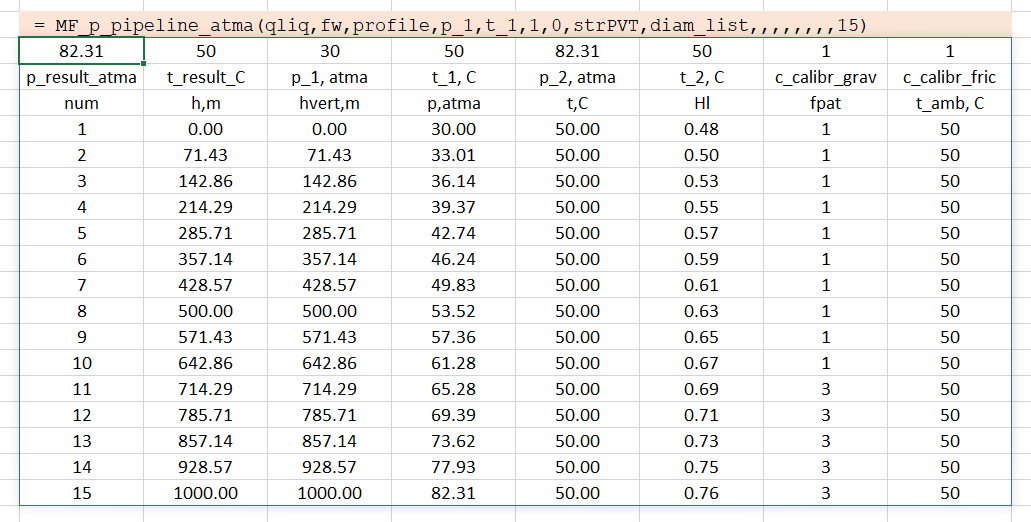
\includegraphics[width=1\linewidth]{pipeline_out_example}
	\caption{Пример вывода результатов расчета функции \mintinline{vb.net}{MF_p_pipeline_atma()}}
	\label{ris:pipeline_out_example}
\end{figure}

\end{comment}

\newpage

